\section{Геометрия задачи}
1. В трапеции $ABCD$ ($AD$ и $BC$ --- основания) диагонали пересекаются в точке $O.$ Доказать, что $S_{\Delta AOB}=S_{\Delta COD}.$\\
2. На стороне $BC$ параллелограмма $ABCD$ взяты произвольные точки $M$ и $K$ так, что отрезки $DM$ и $AK$ пересекаются в точке $O.$ Доказать, что $S_{\Delta AOM}=S_{\Delta KOD}.$\\
3. На каждой медиане равностороннего треугольника $ABC$ взята точка, делящая её в отношении $1:3,$ считая от вершины. Указанные точки обозначим $A_1,\ B_1,\ C_1.$ Найти отношение площадей треугольников $A_1B_1C_1$ и $ABC.$\\
4. На каждой медиане равностороннего треугольника $ABC$ взята точка, делящая её в отношении $1:4,$ считая от вершины. Указанные точки обозначим $A_1,\ B_1,\ C_1.$ Найти отношение площадей треугольников $A_1B_1C_1$ и $ABC.$\\
5. В прямоугольном треугольнике $ABC$ медиана $CM=12$см, а расстояние от середины катета $AC$ до гипотенузы $AB$ равно 3 см. Найдите площадь треугольника $ABC.$\\
6. В прямоугольном треугольнике $ABC$ медиана $CM=8$см, а расстояние от середины катета $AC$ до гипотенузы $AB$ равно 2 см. Найдите площадь треугольника $ABC.$\\
7. Средняя линия трапеции делится двумя диагоналями на три равные части. Найти отношение между основаниями трапеции.\\
8. Средняя линия трапеции равна 8 см и делится диагональю на два отрезка, разность между которыми равна 2 см. Найти основания трапеции.\\
9. Угол, противолежащий основанию равнобедренного треугольника, равен $120^\circ.$ Высота, проведённая к боковой стороне, равна 9 см. Найти основание треугольника.\\
10. Угол, противолежащий основанию равнобедренного треугольника, равен $120^\circ.$ Основание равно 8 см. Найти длину высоты, проведённой к боковой стороне.\\
11. Найти площадь прямоугольной трапеции, у которой две меньшие стороны равны 6 см, а больший угол $135^\circ.$\\
12. Найти площадь прямоугольной трапеции, у которой две меньшие стороны равны 4 см, а меньший угол $45^\circ.$\\
13. Найти углы ромба, если его диагонали равны $2\sqrt{3}$ и $2.$\\
14. Найти углы ромба, если его диагонали равны $4\sqrt{3}$ и $4.$\\
15. К окружности проведены касательная и секущая, проходящая через центр окружности. Длина касательной в два раза меньше длины секущей. Найти отношение длины касательной к длине радиуса.\\
16. К окружности проведены касательная и секущая, проходящая через центр окружности. Длина касательной в три раза меньше длины секущей. Найти отношение длины радиуса окружности к длине касательной.\\
17. Точка $M$ лежит на стороне $BC$ параллелограмма $ABCD,$ причём $BM:MC=3:1.$ Выразите вектор $\overrightarrow{AM}$ через векторы $\overrightarrow{AD}$ и $\overrightarrow{AB}.$\\
18. Точка $M$ лежит на стороне $BC$ параллелограмма $ABCD,$ причём $BM:MC=3:1.$ Выразите вектор $\overrightarrow{MD}$ через векторы $\overrightarrow{AD}$ и $\overrightarrow{AB}.$\\
19. На прямой $l$ найдите точку $C$ такую, чтобы сумма расстояний $AC+BC$ была наименьшей.
$$\begin{tikzpicture}[scale=1]
\tikzset {line01/.style={line width =0.5pt}}
\tikzset{line02/.style={line width =1pt}}
\tikzset{line03/.style={dashed,line width =0.9pt}}
\filldraw [black] (-2.5,1) circle (2pt);
\filldraw [black] (2.8,0.3) circle (2pt);
\draw[line01] (-3,0) -- (3,0);
\draw (2.9,0.6) node {\scriptsize $B$};
\draw (-2.5,0.6) node {\scriptsize $A$};
\draw (3.2,0) node {\scriptsize $l$};
\end{tikzpicture}$$
20. На прямой $l$ найдите точку $C$ такую, чтобы сумма расстояний $AC+BC$ была наименьшей.
$$\begin{tikzpicture}[scale=1]
\tikzset {line01/.style={line width =0.5pt}}
\tikzset{line02/.style={line width =1pt}}
\tikzset{line03/.style={dashed,line width =0.9pt}}
\filldraw [black] (-2.5,-1) circle (2pt);
\filldraw [black] (2.8,-0.3) circle (2pt);
\draw[line01] (-3,0) -- (3,0);
\draw (2.9,-0.6) node {\scriptsize $B$};
\draw (-2.5,-0.6) node {\scriptsize $A$};
\draw (3.2,0) node {\scriptsize $l$};
\end{tikzpicture}$$
21. Дан $ABCD$ --- прямоугольник. $AB=8,\ BC=4.$ На сторонах $AB$ и $CD$ отмечены точки $K$ и $P$ соответственно так, что $AK:AB=CP:CD=3:8.$\\
а) Докажите, что $KBPD$ --- ромб.\\
б) Найдите его периметр и площадь.\\
22. Две окружности, радиусы которых равны 8 и 2, касаются внешним образом. $AB$ --- их общая внешняя касательная ($A$ и $B$ --- точки касания). Найдите длину отрезка $AB.$\\
23. В треугольнике $ABC$ угол $B$ равен $80^\circ.\ M$ --- точка пересечения биссектрис углов $A$ и $C.$ Найти угол $AMC.$\\
24. В треугольнике $ABC$ угол $B$ равен $100^\circ.\ M$ --- точка пересечения биссектрис углов $A$ и $C.$ Найти угол $AMC.$\\
25. Найти диагонали ромба, если одна из них в 1,5 раза больше другой, а площадь ромба равна $27\text{см}^2.$\\
26. Найти диагонали ромба, если одна из них в 2,5 раза больше другой, а площадь ромба равна $20\text{см}^2.$\\
27. Найти площадь четырёхугольника $ABCD,$ если $AB=5,\ BC=13,\ CD=9,\ DA=15$ и $AC=12.$\\
28. Найти площадь четырёхугольника $ABCD,$ если $AB=12,\ BC=8,\ CD=17,\ DA=9$ и $BD=15.$\\
29. В равнобедренной трапеции, описанной  около круга, основания равны 36см и 100см. Найти радиус круга.\\
30. В равнобедренной трапеции, описанной  около круга, основания равны 32см и 50см. Найти радиус круга.\\
31. Из двух пересекающихся хорд одна разделилась на части 48см и 3см, а другая --- пополам. Найти длину второй хорды.\\
32. Из двух пересекающихся хорд одна разделилась на части 16см и 4см, а другая --- пополам. Найти длину второй хорды.\\
33. Два угла равнобедренного треугольника пропорциональны числам 2 и 5. Найдите все углы треугольника.\\
34. Два угла равнобедренного треугольника пропорциональны числам 1 и 4. Найдите все углы треугольника.\\
35. Две стороны треугольника равны 2 и 4. Какие значения может принимать третья сторона, если её длина --- целое число?\\
36. Две стороны треугольника равны 2 и 5. Какие значения может принимать третья сторона, если её длина --- целое число?\\
37. Найдите наибольшую возможную площадь прямоугольного треугольника с гипотенузой 10см.\\
38. Найдите наибольшую возможную площадь прямоугольного треугольника с гипотенузой 12см.\\
39. Равнобедренный треугольник, углы которого относятся как $4:1,$ достроили до параллелограмма, диагональю которого является боковая сторона. Найти углы параллелограмма.\\
40. Равнобедренный треугольник, углы которого относятся как $5:2,$ достроили до параллелограмма, диагональю которого является боковая сторона. Найти углы параллелограмма.\\
41. В треугольнике $ABC\ BC=34$см. Перпендикуляр $MN,$ проведённый из середины $BC$ к прямой $AC,$ делит сторону $AC$ на отрезки $AN=25$см и $NC=15$см. Найти площадь треугольника $ABC.$\\
42. В треугольнике $ABC\ BC=26$см. Перпендикуляр $MN,$ проведённый из середины $BC$ к прямой $AC,$ делит сторону $AC$ на отрезки $AN=19$см и $NC=5$см. Найти площадь треугольника $ABC.$\\
43. Найти радиус окружности, вписанной в прямоугольную трапецию с основаниями 4 и 6.\\
44. Найти радиус окружности, вписанной в прямоугольную трапецию с основаниями 2 и 3.\\
45. Найдите длину медианы $CM$ треугольника $ABC,$ если известны координаты вершин треугольника: $A(2;-5),\ B(4;-3),\ C(0;0).$\\
46. Найдите длину медианы $CM$ треугольника $ABC,$ если известны координаты вершин треугольника: $A(-2;5),\ B(-4;3),\ C(0;0).$\\
47. Основания трапеции равны 12 см и 18 см. Найти длины отрезков, на которые диагонали трапеции делят её среднюю линию.\\
48. Основания трапеции равны 10 см и 16 см. Найти длины отрезков, на которые диагонали трапеции делят её среднюю линию.\\
49. Найти периметр параллелограмма, если его площадь равна 24 кв. см., а точка пересечения диагоналей удалена от его сторон на 2 и 3 см.\\
50. Найти периметр параллелограмма, если его площадь равна 48 кв. см., а точка пересечения диагоналей удалена от его сторон на 3 и 4 см.\\
51. Катеты прямоугольного треугольника относятся как $3:4,$ гипотенуза равна 50. Найти отрезки, на которые гипотенуза делится высотой, проведённой из вершины прямого угла.\\
52. Катет прямоугольного треугольника относится к гипотенузе, равной 25 см, как $3:5.$ Найти отрезки, на которые гипотенуза делится высотой, проведённой из вершины прямого угла.\\
53. Стороны треугольник 5 см, 12 см и 13 см. Найти длину медианы, проведённой к большей стороне.\\
54. Стороны треугольник 6 см, 8 см и 10 см. Найти длину медианы, проведённой к большей стороне.\\
55. В прямоугольном треугольнике $ABC$ угол $C$ прямой, $tg A=\cfrac{1}{2}.$ Найдите $\cos A.$\\
56. В прямоугольном треугольнике $ABC$ угол $C$ прямой, $tg A=\cfrac{2}{3}.$ Найдите $\cos A.$\\
57. Периметр параллелограмма равен 18 см, а одна из его высот в два раза больше другой. Найти стороны параллелограмма.\\
58. Периметр прямоугольника равен 28 см, а диагональ 10 см. Найти стороны прямоугольника.\\
59. Сумма внутренних углов многоугольника в 2 раза больше суммы внутренних углов квадрата. Найти число сторон многоугольника.\\
60. Сумма внутренних углов многоугольника в 3 раза больше суммы внутренних углов квадрата. Найти число сторон многоугольника.\\
61. В треугольнике $ABC$ на стороне $AC$ взяли точку $M$ и провели прямую, параллельную $AB,$ которая пересекла сторону $BC$ в точке $N.$ Найдите отношение площади треугольника $MCN$ к площади трапеции $AMNB,$ если $AM:MC=2:3.$\\
62. В треугольнике $ABC$ на стороне $AC$ взяли точку $M$ и провели прямую, параллельную $AB,$ которая пересекла сторону $BC$ в точке $N.$ Найдите отношение площади треугольника $MCN$ к площади трапеции $AMNB,$ если $AM:MC=3:2.$\\
63. Периметр прямоугольника 34 см, а диагональ 13 см. Найти стороны прямоугольника.\\
64. В прямоугольной трапеции основания равны 2 см и 6 см. Меньшая боковая сторона равна 3 см. Найти косинус острого угла.\\
65. В прямоугольной трапеции основания равны 5 см и 8 см. Меньшая боковая сторона равна 4 см. Найти косинус острого угла.\\
66. В треугольнике $ABC$ углы $A$ и $B$ равны соответственно $48^\circ$ и $76^\circ.$ Найдите угол между биссектрисой и высотой, проведёнными из вершины $C.$\\
67. В треугольнике $ABC$ углы $B$ и $C$ равны соответственно $64^\circ$ и $24^\circ.$ Найдите угол между биссектрисой и высотой, проведёнными из вершины $A.$\\
68. На стороне $AB$ параллелограмма $ABCD$ отметили точку $M.$ Площадь треугольника $MCD$ равна $38\text{см}^2.$ Найдите площадь параллелограмма.\\
69. На стороне $AD$ параллелограмма $ABCD$ отметили точку $M.$ Площадь треугольника $MCB$ равна $42\text{см}^2.$ Найдите площадь параллелограмма.\\
70. Расстояние от вершины квадрата до середины стороны, не содержащей эту вершину, равно 3 см. Найдите площадь квадрата.\\
71. Расстояние от вершины квадрата до середины стороны, не содержащей эту вершину, равно 4 см. Найдите площадь квадрата.\\
72. В прямоугольный треугольник вписана окружность, которая точкой касания делит гипотенузу на 2 части --- 2 см и 3 см. Найдите радиус окружности.\\
73. В прямоугольный треугольник вписана окружность, которая точкой касания делит гипотенузу на 2 части --- 4 см и 6 см. Найдите радиус окружности.\\
74. Площадь прямоугольной трапеции $54\text{см}^2.$ Две меньшие стороны равны между собой, а острый угол равен $45^\circ.$ Найти меньшее основание.\\
75. Площадь прямоугольной трапеции $24\text{см}^2.$ Две меньшие стороны равны между собой, а острый угол равен $45^\circ.$ Найти меньшее основание.\\
76. Сторона ромба равна 10, а одна из диагоналей 12. Найти вторую диагональ.\\
77. Сторона ромба равна 10, а одна из диагоналей 16. Найти вторую диагональ.\\
78. В равнобедренном треугольнике с углом $70^\circ$ при вершине найти угол между высотами, проведёнными к боковым сторонам.\\
79. В равнобедренном треугольнике с углом $50^\circ$ при вершине найти угол между высотами, проведёнными к боковым сторонам.\\
80. Диагональ $AC$ параллелограмма $ABCD$ равна 18. Середина $M$ стороны $AB$ соединена с точкой $D.$ Найти отрезки, на которые диагональ $AC$ делится отрезком $DM.$\\
81. Диагональ $AC$ параллелограмма $ABCD$ равна 15. Середина $M$ стороны $AB$ соединена с точкой $D.$ Найти отрезки, на которые диагональ $AC$ делится отрезком $DM.$\\
82. В прямоугольном треугольнике угол $C$ прямой, катет $AC$ равен $m,\ \angle CAB$ равен $\alpha.$ Найти катет $BC.$\\
83. В прямоугольном треугольнике угол $C$ прямой, катет $AC$ равен $m,\ \angle ABC$ равен $\alpha.$ Найти катет $BC.$\\
84. Диагонали ромба 14 см и 13 см. Найдите его площадь.\\
85. Диагонали ромба 16 см и 11 см. Найдите его площадь.\\
86. Около прямоугольного треугольника $ABC$ с прямым углом $C$ описана окружность. Найдите радиус этой окружности, если $AC=18\text{ см,}\ \angle B=30^\circ.$\\
87. Около прямоугольного треугольника $ABC$ с прямым углом $C$ описана окружность. Найдите радиус этой окружности, если $BC=12\text{ см,}\ \angle A=30^\circ.$\\
88. В прямоугольном треугольнике угол $C$ прямой, $\sin \angle A=\cfrac{2}{3}.$ Найдите тангенс этого угла.\\
89. В прямоугольном треугольнике угол $C$ прямой, $\cos \angle A=\cfrac{2}{3}.$ Найдите тангенс этого угла.\\
90. В равнобедренном треугольнике угол между высотами, проведёнными к боковым сторонам, равен $40^\circ.$ Найдите угол при вершине треугольника.\\
91. В равнобедренном треугольнике угол между высотами, проведёнными к боковым сторонам, равен $80^\circ.$ Найдите угол при вершине треугольника.\\
92. В четырёхугольнике $ABCD$ точки $M,\ N,\ P,\ Q$ --- середины сторон. Найдите площадь четырёхугольника $MNPQ,$ если площадь четырёхугольника $ABCD$ равна $S.$\\
93. В четырёхугольнике $ABCD$ точки $M,\ N,\ P,\ Q$ --- середины сторон. Найдите площадь четырёхугольника $ABCD,$ если площадь четырёхугольника $MNPQ$ равна $S.$\\
94. В треугольнике $ABC$ угол $C$ прямой, $AC=3,\ BC=4.$ Найдите медиану $CK.$\\
95. Три окружности, радиусы которых 2, 4 и 6, попарно касаются внешним образом. Найдите радиус окружности, вписанной в треугольник, вершинами которого являются центры этих трёх окружностей.\\
96. Сторона ромба равна 20, а тупой угол $120^\circ.$ Найдите длину меньшей диагонали.\\
97. Гипотенуза $AB$ прямоугольного треугольника $ABC$ равна $c,$ а мера острого угла $A$ равна $\alpha.$ Найти периметр треугольника.\\
98. Гипотенуза $AB$ прямоугольного треугольника $ABC$ равна $c,$ а мера острого угла $A$ равна $\alpha.$ Найти площадь треугольника.\\
99. В трапеции большее основание равно 18 см, углы при большем основании равны $53^\circ$ и $37^\circ.$ Найти расстояние от точки пересечения боковых сторон до середины большего основания.\\
100. В трапеции большее основание равно 22 см, углы при большем основании равны $58^\circ$ и $32^\circ.$ Найти расстояние от точки пересечения боковых сторон до середины большего основания.\\
101. Две окружности, радиусы которых отличаются в 4 раза, касаются внешним образом. $AB$ --- их общая касательная ($A$ и $B$ --- точки касания) имеет длину 8 см. Найти радиусы окружностей.\\
102. Две окружности, радиусы которых отличаются в 4 раза, касаются внешним образом. $AB$ --- их общая касательная ($A$ и $B$ --- точки касания) имеет длину 16 см. Найти радиусы окружностей.\\
103. В равнобедренном треугольнике один из углов равен $120^\circ,$ а высота, проведённая к боковой стороне, равна 15 см. Найдите основание треугольника.\\
104. В равнобедренном треугольнике один из углов равен $120^\circ.$ Найти высоту, проведённую к боковой стороне стороне, если основание треугольника равно 30 см.\\
105. Четырёхугольник $ABCD$ --- трапеция $(AD\parallel BC).$ Известно, что $\cfrac{S_{\Delta AOD}}{S_{\Delta BOC}}=16.$ Найти $\cfrac{BC}{AD}.$\\
106. Четырёхугольник $ABCD$ --- трапеция $(AD\parallel BC).$ Известно, что $\cfrac{S_{\Delta AOD}}{S_{\Delta BOC}}=25.$ Найти $\cfrac{BC}{AD}.$\\
107. Стороны треугольника равны $\sqrt{2},\ \sqrt{7},\ 3.$ Найдите площадь треугольника.\\
108. Стороны треугольника равны $\sqrt{5},\ \sqrt{11},\ 4.$ Найдите площадь треугольника.\\
109. В прямоугольной трапеции $ABCD$ $(AD\parallel BC),$ угол $B=120^\circ,\ AB=BC=4.\ K$ --- середина $BC.$ Найти $AK.$\\
110. В прямоугольной трапеции $ABCD$ $(AD\parallel BC),$ угол $B=120^\circ,\ AB=BC=6.\ K$ --- середина $BC.$ Найти $AK.$\\
111. В прямоугольном треугольнике с прямым углом $B$ проведена высота $BH.$ Найдите $AH,$ если $\angle ABH=60^\circ$ и $CH=8.$\\
112. В прямоугольном треугольнике с прямым углом $B$ проведена высота $BH.$ Найдите $HC,$ если $\angle ACB=60^\circ$ и $AH=12.$\\
113. В прямоугольном треугольнике с прямым углом $B$ проведена высота $BH.$ Найдите $AH,$ если $\angle ABH=60^\circ$ и $CH=4.$\\
114. В прямоугольном треугольнике с прямым углом $B$ проведена высота $BH.$ Найдите $HC,$ если $\angle ACB=60^\circ$ и $AH=18.$\\
115. Найдите площадь трапеции со взаимно перпендикулярными диагоналями длины 4 и 5.\\
116. Найдите площадь трапеции со взаимно перпендикулярными диагоналями длины 8 и 5.\\
117. Найдите площадь трапеции со взаимно перпендикулярными диагоналями длины 6 и 7.\\
118. Найдите площадь трапеции со взаимно перпендикулярными диагоналями длины 6 и 5.\\
119. В прямоугольнике $ABCD$ на стороне $AD$ взята точка $L,$ а на стороне $BC$ взята точка $K$ так, что $KD=DL=KL=6,\ \angle ABL=60^\circ.$ Найдите площадь прямоугольника.\\
120. В прямоугольнике $ABCD$ на стороне $AD$ взята точка $L,$ а на стороне $BC$ взята точка $K$ так, что $KD=DL=KL=8,\ \angle ABL=45^\circ.$ Найдите площадь прямоугольника.\\
121. В прямоугольнике $ABCD$ на стороне $AD$ взята точка $L,$ а на стороне $BC$ взята точка $K$ так, что $KD=DL=KL=8,\ \angle ABL=60^\circ.$ Найдите площадь прямоугольника.\\
122. В прямоугольнике $ABCD$ на стороне $AD$ взята точка $L,$ а на стороне $BC$ взята точка $K$ так, что $KD=DL=KL=6,\ \angle ABL=45^\circ.$ Найдите площадь прямоугольника.\\
123. В треугольнике $ABC$ биссектриса угла $A$ пересекает биссектрису угла, смежного с углом $C,$ в точке $M.$ Найдите расстояние от точки $M$ до прямой $AB,$ если расстояние от точки $M$ до прямой $BC$ равно 4.\\
124. В четырёхугольнике $ABCD: AD=BC,$ серединные перпендикуляры к сторонам $AB$ и $CD$ пересекаются в точке $P.$ Найдите угол $BCP,$ если $\angle ADP=30^\circ.$\\
125. В треугольнике $ABC$ через точку пересечения биссектрис углов $A$ и $B$ проведена прямая, параллельная $AB,$ пересекающая стороны треугольника в точках $K$ и $N.$ Найдите длину $AB,$ если периметр треугольника $ABC$ равен 12, а периметр треугольника $KCN$ равен 8.\\
126. В треугольнике $ABC$ через точку пересечения биссектрис углов, смежных с углами $A$ и $B,$ проведена прямая, параллельная $AB,$ пересекающая продолжения сторон треугольника в точках $K$ и $N.$ Найдите длину $AB,$ если периметр треугольника $CKN$ равен 22, периметр $ABC$ равен 18, а длина $KN$ равна 4.\\
127. В треугольнике $ABC\ AB:AC=3:5,\ AD$ --- биссектриса. Найдите площадь треугольника $ACD,$ если площадь треугольника $ABD$ равна $9\text{см}^2.$\\  128. В треугольнике $ABC\ BM$ --- биссектриса. Площадь треугольника $ABM$ относится к площади треугольника $BCM$ как $1:3.$ Найдите $AB,$ если $BC$ --- 12 см.\\
129. Точка $K$ принадлежит стороне $AB$ параллелограмма $ABCD.$ Найдите площадь $ABCD,$ если площадь треугольника $CDK$ равна 28.\\
130. Точка $L$ принадлежит стороне $BC$ параллелограмма $ABCD.$ Найдите площадь $ABCD,$ если площадь треугольника $ALD$ равна 23.\\
131. В остроугольном треугольнике $ABC$ провели высоты $AA_1$ и $BB_1.$ Найдите $\angle CA_1B_1,$ если $\angle BAC=32^\circ.$\\
132. В остроугольном треугольнике $ABC$ провели высоты $AA_1$ и $BB_1.$ Найдите $\angle CB_1A_1,$ если $\angle CBA=17^\circ.$\\
133. В трапеции $ABCD$ основание $AD$ больше основания $BC$ на 5 см. Найдите длину отрезка, соединяющего середины оснований, если $\angle A=12^\circ,\ \angle D=78^\circ.$\\
134. В трапеции $ABCD$ основание $AD$ больше основания $BC$ на 3 см. Найдите длину отрезка, соединяющего середины оснований, если $\angle A=21^\circ,\ \angle D=69^\circ.$\\
135. Найдите острые углы прямоугольного треугольника, если его гипотенуза --- 12, а высота, проведённая к ней, равна 3.\\
136. Найдите острые углы прямоугольного треугольника, если его гипотенуза --- 16, а высота, проведённая к ней, равна 4.\\
137. Разность углов, прилегающих к одной стороне параллелограмма, равна $48^\circ.$ Найдите больший угол параллелограмма.\\
138. Разность углов, прилегающих к одной стороне параллелограмма, равна $54^\circ.$ Найдите больший угол параллелограмма.\\
139. Вокруг равностороннего треугольника $ABC$ описана окружность радиуса 10. Найдите радиус вписанной окружности.\\
140. Вокруг равностороннего треугольника $ABC$ описана окружность радиуса 8. Найдите радиус вписанной окружности.\\
141. В прямоугольный треугольник вписана окружность. Точка касания делит гипотенузу на отрезки 3 и 2. Найти радиус окружности.\\
142. В прямоугольный треугольник вписана окружность. Точка касания делит гипотенузу на отрезки 4 и 6. Найти радиус окружности.\\
143. Высота равнобедренного треугольника $ABC,$ опущенная из вершины $B$ на основание $AC$ равна $a,$ угол $A=\alpha.$ Найдите площадь треугольника.\\
144. Основание $AC$ равнобедренного треугольника $ABC$ равно $a,$ угол $A=\alpha.$ Найдите площадь треугольника.\\
145. Дан треугольник $OAB: O(0;0),\ A(2;2),\ B(x;2).$ Найдите координаты точки $B,$ если площадь треугольника $OAB=4.$\\
146. Дан треугольник $OAB: O(0;0),\ A(4;4),\ B(x;4).$ Найдите координаты точки $B,$ если площадь треугольника $OAB=4.$\\
147. Найдите большую высоту треугольника со сторонами $3\sqrt{3},\ \sqrt{11},\ 4.$\\
148. Найдите большую высоту треугольника со сторонами $4\sqrt{3},\ \sqrt{23},\ 5.$\\
149. В треугольнике $ABC$ проведена прямая $BD$ так, что угол $ABD$ равен углу $C.$ Найдите отрезки $AD$ и $DC,$ если $AB=2,\ AC=4.$\\
150. В трапеции диагональ и боковая сторона, выходящие из вершины тупого угла, равны 26 см и $\sqrt{577}$ см соответственно, высота трапеции 24 см, меньшее основание 7 см. Найдите площадь трапеции.\\
151. Дан прямоугольный треугольник $ABC,$ в котором $tg\angle A=\cfrac{1}{2}.$ Найдите $\cos \angle A.$\\
152. В квадрате $ABCD: AB=16,\ K$ --- середина $BC,\ M$ лежит на стороне $CD,$ причём $KM=AM.$ Найдите $MD.$\\
153. В квадрате $KLMN: KL=8,\ B$ --- середина $MN,\ A$ лежит на стороне $KN,$ причём $LA=AB.$ Найдите $AN.$\\
154. В трапеции $KLMN$ с основанием $LM$ точка $Q$ принадлежит отрезку $KN,$ причём $(MQ)\parallel(LK).$ Найдите $S(KLMN),$ если $S(QMN)=21,\ LM:KN=4:7.$\\
155. В трапеции $ABCD$ с основанием $AD$ точка $K$ принадлежит отрезку $AD,$ причём $(BK)\parallel(CD).$ Найдите $S(ABCD),$ если $S(BKC)=15,\ BC:AD=5:12.$\\
156. Биссектриса угла $A$ трапеции $ABCD$ с основанием $AD$ пересекает $CD$ в точке $K,$ делящей отрезок $CD$ пополам. Найдите $AB,$ если $BC=4,\ AD=10.$\\
157. В трапеции $ABCD$ точка $K$ --- середина боковой стороны $CD,\ \angle BAK=\angle ABK.$ Найдите $\angle BAD.$\\
158. В прямоугольном треугольнике $ABC$ известны длины катетов $AC=3,\ BC=4.\ O$ --- центр вписанной окружности. Найти:\\
а) Радиус вписанной окружности;\\
б)$\angle AOB;$\\
в) Площадь треугольника $BCK,$ где $BK$ --- биссектриса треугольника $ABC.$\\
159. Основания трапеции равны 10 см и 4 см, а углы при большем основании составляют $30^\circ$ и $60^\circ.$\\
а) Найдите боковые стороны трапеции;\\
б) Найдите площадь трапеции;\\
в) Найти длину отрезка, соединяющего середины оснований трапеции.\\
160. В треугольнике $ABC\ BC=1,\ \angle A=30^\circ.$ Найти наибольшую возможную длину стороны $AB.$\\
161. Какую наибольшую площадь может иметь прямоугольный треугольник, вписанный в окружность радиуса 1?\\
162. В трапеции $ABCD$ с основаниями $AD$ и $BC\ \angle A=60^\circ,\ \angle D=30^\circ,\ AB=BC=2.$ Найти:\\
а) $CD;$\\
б) Площадь трапеции $ABCD;$\\
в) Площадь треугольника $AOD,$ если диагонали трапеции пересекаются в точке $O;$\\
г) Расстояние между серединами сторон $AD$ и $BC.$\\
163. Дан отрезок длины 1. Пользуясь циркулем и линейкой, построить отрезок длины $\sqrt{7}.$\\
164. Периметр прямоугольника равен 1 м, а площадь равна $616\text{см}^2.$ Найдите площадь ромба, один из углов которого равен $60^\circ,$ а сторона равна меньшей из сторон прямоугольника.\\
165. Через вершину $C$ равностороннего треугольника $ABC$ проведена прямая, пересекающая сторону $AB.$ Расстояния от этой прямой до точек $A$ и $B$ соответственно равны 1 и 7. Найдите стороны треугольника.\\
166. Трапеция $ABCD$ вписана в окружность. Угол $A$ равен $60^\circ,$ угол $ABD$ равен $90^\circ,\ CD=4$см. Найти:\\
а) Определить вид трапеции;\\
б) Радиус этой окружности;\\
в) Площадь треугольника $ABD;$\\
г) Площадь треугольника $BCD.$\\
167. В трапеции $ABCD$ с основаниями $AD$ и $BC$ диагонали пересекаются в точке $O,\ \angle A=60^\circ,\ AB=BC=6,\ AD=18.$ Найдите:\\
а) Длину стороны $CD;$\\
б) Величину угла $ACD;$\\
в) Площадь треугольника $AOB;$\\
г) Длину отрезка с концами на боковых сторонах трапеции, проходящего через точку $O$ и параллельного основаниям.\\
168. Дан отрезок длины 1. Пользуясь циркулем и линейкой, построить отрезок длины $\sqrt{6}.$\\
169. Пусть $ABCD$ --- выпуклый четырёхугольник, $O$ --- точка пересечения его диагоналей, $OB=OD,\ AO<OC.$ Докажите, что $\angle BAD > \angle BCD.$\\
170. В равнобедренном треугольнике длина основания равна 4, а длина медианы, проведённой к боковой стороне, равна 5. Найдите площадь треугольника.\\
171. Отрезки, соединяющие середины противоположных стороны выпуклого четырёхугольника, равны, длины диагоналей этого четырёхугольника равны 6 и 8. Найдите площадь четырёхугольника.\\
172. В трапеции $ABCD\ (AD\parallel BC)\ \angle A=60^\circ,\ \angle D=30^\circ,\ AD=a,\ BC=b.$ Найдите:\\
а) Площадь трапеции $ABCD;$\\
б) Длину отрезка, соединяющего середины $BC$ и $AD.$\\
173. В трапеции $ABCD$ с основаниями $AD$ и $BC$ диагонали пересекаются в точке $O,$ которая удалена от прямой $CD$ на 6 см. Найдите площадь треугольника $AOB,$ если $CD=8$см.\\
174. Окружность пересекает стороны $AB$ и $AC$ треугольника $ABC$ в точках $K$ и $P$ соответственно и проходит через вершины $B$ и $C.$ Найдите длину отрезка $KP,$ если $AK=6$см, а сторона $AC$ в 1,5 раза больше стороны $BC.$\\
175. Найти площадь треугольника с вершинами, расположенными в точках $(1;8),\ (5;7),\ (7;2)$ координатной плоскости.\\
176. Диагональ $AC$ параллелограмма $ABCD$ равна 24 см. Середина $M$ стороны $AB$ соединена с вершиной $D.$ Найдите отрезки, на которые делится диагональ $AC$ отрезком $DM.$\\
177. В прямоугольном треугольнике $ABC$ с катетами $AC$ и $BC$ угол $A$ равен $60^\circ.$ Биссектриса угла $A$ пересекает катет $BC$ в точке $P,$ длина отрезка $PB$ равна 4. Найдите\\
а) площадь треугольника $ABC;$\\
б) площадь треугольника $ABP;$\\
в) радиус окружности, описанной вокруг треугольника $ABP.$\\
178. В прямоугольном треугольнике $ABC$ с катетами $AC$ и $BC$ угол $A$ равен $60^\circ.$ Биссектриса угла $A$ пересекает катет $BC$ в точке $P,$ длина отрезка $PC$ равна 1. Найдите\\
а) площадь треугольника $ABC;$\\
б) площадь треугольника $ABP;$\\
в) радиус окружности, описанной вокруг треугольника $ABP.$\\
179. Найдите площадь равнобедренной трапеции, основания которой равны 12 см и 6 см, а один из углов равен 60 градусов.\\
180. В остроугольном треугольнике $ABC$ его высоты $BD$ и $AE$ пересекаются в точке $O.$ Докажите, что $BO\cdot OD=AO\cdot OE.$\\
181. Диагональ $BD$ параллелограмма $ABCD$ является его высотой, опущенной на AD, и равна половине стороны $AB.$ Найдите расстояние между прямыми $AB$ и $CD,$ если $AD = 8.$\\
182. Диагональ $BD$ параллелограмма $ABCD$ является его высотой, опущенной на $AD,$ и равна половине стороны $AB.$ Найдите расстояние между прямыми $AB$ и $CD,$ если $BC = 4.$\\
183. Известны длины сторон $\Delta ABC:\ AB = 5,\ CA = 8,\  BC = 9.$ На луче $AB,$ за точкой $B,$ выбрана такая точка $K,$ что $\angle KCA = \angle ABC.$ Найдите стороны $\Delta KBC.$\\
184. Известны длины сторон $\Delta ABC:\ AB = 4,\ AC = 8,\  BC = 6.$ На отрезке $BC$ выбрана такая точка $D,$ что $\angle BAD = \angle ACB.$ Найдите стороны $\Delta ADC.$\\
185. Медианы треугольника $ABC,$ проведённые из вершин $B$ и $C,$ пересекаются под прямым углом. Найдите $|BC|,$ если длина медианы треугольника, проведённой из вершины $A,$ равна 36.\\
186. Медианы треугольника $ABC,$ проведённые из вершин $B$ и $C,$ пересекаются под прямым углом. Найдите длину медианы треугольника, проведённой из вершины $A,$ если $|BC| = 42.$\\
187. На чертеже --- параллелограмм. Подписаны площади его отдельных частей. Определите площадь треугольника, отмеченного знаком вопроса.
\begin{figure}[ht!]
\center{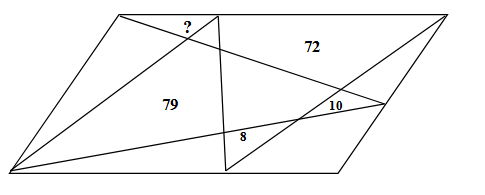
\includegraphics[scale=0.6]{06.png}}
\end{figure}\\
188. На чертеже --- параллелограмм. Подписаны площади его отдельных частей. Определите площадь четырёхугольника, отмеченного знаком вопроса.
\begin{figure}[ht!]
\center{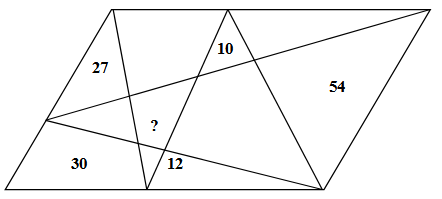
\includegraphics[scale=0.6]{07.png}}
\end{figure}\\
189. Найдите стороны параллелограмма $ABCD,$ если его периметр равен 64 см, а биссектриса острого угла $A$ делит сторону $BC$ в отношении 1:2, считая от вершины $B.$\\
190. Найдите стороны параллелограмма $ABCD,$ если его периметр равен 100 см, а биссектриса острого угла $A$ делит сторону $BC$ в отношении 2:1, считая от вершины $B.$\\
191. Найдите меньшую высоту треугольника со сторонами, равными 15см , 17см, 8см.\\
192. Найдите меньшую высоту треугольника со сторонами, равными 24см, 25см, 7см.\\
193. Разность двух оснований равнобедренной трапеции равна 3. Синус угла при ее основании равен 0,8. Найдите длину боковой стороны трапеции.\\
194. Разность двух оснований равнобедренной трапеции равна 4. Синус угла при ее основании равен 0,6. Найдите длину боковой стороны трапеции.\\
195. Две стороны равнобедренного треугольника равны равны 3 см и 7 см. Найдите третью сторону. Ответ обосновать.\\
196. Две стороны равнобедренного треугольника равны равны 2 см и 5 см. Найдите третью сторону. Ответ обосновать.\\
197. Периметр равнобедренного треугольника равен 18 см и одна из его сторон меньше другой на 6 см. Найти стороны треугольника.\\
198. Периметр равнобедренного треугольника равен 27 см и одна из его сторон меньше другой на 9 см. Найти стороны треугольника.\\
199. В равносторонний треугольник вписана окружность радиуса 4. Найти радиус описанной окружности.\\
200. В равносторонний треугольник вписана окружность радиуса 6. Найти радиус описанной окружности.\\
201. Точка $O$ --- точка пересечения медиан $AM$ и $BK$ треугольника $ABC.$ Сравните площади треугольников $AOK$ и $BOM.$ Ответ обосновать.\\
202. $ABCD$ трапеция с основаниями $AD$ и $BC.$ Точка $O$ --- точка пересечения диагоналей трапеции. Сравните площади треугольников $ABO$ и $DCO.$ Ответ обосновать.\\
203. Углы $A$ и $B$ и треугольника $ABC$ равны соответственно $71^\circ$ и $79^\circ.$ Найдите $AB,$ если радиус окружности, описанной около треугольника $ABC,$ равен 8.\\
204. Углы $B$ и $C$ и треугольника $ABC$ равны соответственно $81^\circ$ и $69^\circ.$ Найдите $BC,$ если радиус окружности, описанной около треугольника $ABC,$ равен 5.\\
205. В равнобедренной трапеции диагональ делит тупой угол пополам. Найдите большее основание трапеции, если его длина на 25 см меньше периметра, а средняя линия равна 8 см.\\
206. В равнобедренной трапеции диагональ делит тупой угол пополам. Найдите большее основание трапеции, если его длина на 31 см меньше периметра, а средняя линия равна 10 см.\\
207. В прямоугольном треугольнике $ABC$ (угол $C$ прямой) $tg\; A=2.$ Найти $\cfrac{\sin A -\cos A}{\sin A +\cos A}.$\\
208. В прямоугольном треугольнике $ABC$ (угол $C$ прямой) $tg\; A=3.$ Найти $\cfrac{\sin A +\cos A}{\sin A - \cos A}.$\\
209. В параллелограмме $ABCD$ на продолжении стороны $DC$ взята точка $M$ так, что $DM=3DC.$ (Точка $C$
лежит между $D$и $M).\ K$ --- точка пересечения прямых $AM$ и $BC.$ Найдите площадь треугольника $ABK,$ если
площадь параллелограмма равна 12.\\
210. В параллелограмме $ABCD$ на продолжении стороны $DC$ взята точка $M$ так, что $DM=4DC.$ (Точка $C$
лежит между $D$и $M).\ K$ --- точка пересечения прямых $AM$ и $BC.$ Найдите площадь треугольника $ABK,$ если
площадь параллелограмма равна 16.\\
211. В треугольнике $ABC$ угол $B$ равен $80^\circ.\ M$ --- точка пересечения биссектрис углов $A$ и $C.$
Найдите угол между биссектрисами треугольника.\\
212. В треугольнике $ABC$ угол $B$ равен $100^\circ.\ M$ --- точка пересечения биссектрис углов $A$ и $C.$
Найдите угол между биссектрисами треугольника.\\
213. Две стороны треугольника равны 2 и 4. Какие значения может принимать третья сторона, если её длина --- целое число?\\
214. Две стороны треугольника равны 2 и 5. Какие значения может принимать третья сторона, если её длина --- целое число?\\
215. Периметр параллелограмма равен 70 см, а его высоты 3 см и 4 см. Найдите стороны параллелограмма.\\
216. Стороны параллелограмма равны 15 см и 30 см, расстояние между меньшими сторонами --- 20 см. Найдите расстояние между большими сторонами параллелограмма.\\
217. Найдите площадь параллелограмма $ABCD,$ в котором угол $A$ равен $60^\circ,$ а биссектриса $AE$ делит сторону $BC$ на отрезки $BE=2$ и $EC=1.$\\
218. Найдите площадь параллелограмма $ABCD,$ в котором угол $A$ равен $60^\circ,$ а биссектриса $AE$ делит сторону $BC$ на отрезки $BE=1$ и $EC=3.$\\
219. В треугольнике $ABC$ проведена высота $CD.$ Известно, что $CD^2=AD\cdot DB.$\\
а) Докажите, что если точка $D$ лежит на отрезке $AB,$ то треугольник $ABC$ прямоугольный.\\
б) Возможно ли такое соотношение в случае, если $D$ не лежит на отрезке $AB?$ Если да --- приведите пример, если нет --- докажите, почему.\\
220. В треугольнике $ABC$ проведена высота $CH.$ Известно, что $CH^2=AH\cdot HB.$\\
а) Докажите, что если точка $H$ лежит на отрезке $AB,$ то треугольник $ABC$ прямоугольный.\\
б) Возможно ли такое соотношение в случае, если $H$ не лежит на отрезке $AB?$ Если да --- приведите пример, если нет --- докажите, почему.\\
221. Дана равнобедренная трапеция с основаниями 1 и 3. Определить, верно или неверно утверждение (и объяснить, почему):\\
1) если высота равна 1, то диагональ больше, чем 3;\\
2) если диагональ больше, чем 3, то угол при основании больше, чем $45^\circ;$\\
3) если боковая сторона больше 2, то площадь больше 4;\\
4) если площадь равна 1, то радиус описанной окружности больше 1.\\
222. Докажите, что не существует треугольника со сторонами $\sqrt{2}$см, 4 см и $\sqrt{5}$ см.\\
223. На большем основании $AD$ трапеции $ABCD$ взята точка $N$ так, что $AN:ND=3:1.$ Найти $S(\Delta ACD),$ если $S(\Delta ABN)=6.$\\
224. Из середины каждой стороны остроугольного $\Delta ABC$ опущены перпендикуляры на две другие стороны треугольника. Найти площадь ограниченного ими шестиугольника, если $S(\Delta ABC)=8.$\\
225. В равнобедренной трапеции даны: длина меньшего основания трапеции --- $a,$ высота трапеции --- $h,$ острый угол трапеции --- $\alpha.$ Найдите периметр, среднюю линию и площадь этой трапеции.\\
226. В равнобедренной трапеции даны: длины оснований трапеции --- $a$ и $b\ (a<b),$ острый угол трапеции --- $\alpha.$ Найдите периметр, высоту и площадь этой трапеции.\\
227. На сторонах $AB$ и $AC$ треугольника $ABC$ соответственно выбрали точки $D$ и $E$ так, что $DE\parallel BC.$ Оказалось, что $AE=4,\ ED=5,\ DB=6,\ BC=20.$ Найдите периметр и площадь четырёхугольника $BDEC.$\\
228. На сторонах $AD$ и $AE$ треугольника $ADE$ соответственно выбрали точки $C$ и $B$ так, что $BC\parallel DE.$ Оказалось, что $AB=5,\ BC=6,\ CD=4,\ DE=18.$ Найдите периметр и площадь четырёхугольника $BCDE.$\\
229. Пусть $CH$ --- высота прямоугольного треугольника $ABC,$ проведённая к гипотенузе, $AH=9$см, $BC=20$см. Найдите площадь треугольника $ABC.$\\
230. Пусть $CH$ --- высота прямоугольного треугольника $ABC,$ проведённая к гипотенузе, $BH=16$см, $AC=15$см. Найдите площадь треугольника $ABC.$\\
231. На стороне $BC$ параллелограмма $ABCD$ выбрана точка $K$ так, что $BK:CK=5:2.$ Отрезок $KD$ пересекает диагональ $AC$ параллелограмма в точке $M.$ Луч $BM$ пересекает отрезок $CD$ в точке $P.$ Найдите отношение $CP:PD.$\\
232. На стороне $AD$ параллелограмма $ABCD$ выбрана точка $P$ так, что $AD:DP=4:3.$ Отрезок $PC$ пересекает диагональ $BD$ параллелограмма в точке $K.$ Луч $AK$ пересекает отрезок $CD$ в точке $M.$ Найдите отношение $CM:MD.$\\
233. Найдите периметр равнобедренного треугольника, если две его стороны равны 4 см и 9 см. Если ответов существует больше одного, в ответ запишите их сумму.\\
234. Найдите периметр равнобедренного треугольника, если две его стороны равны 5 см и 10 см. Если ответов существует больше одного, в ответ запишите их сумму.\\
235. В четырёхугольнике $ABCD$ известно, что $\angle A=90^\circ,\ \angle B=120^\circ,\ \angle D=30^\circ,\ AB=6,\ BC=4.$ Найдите $CD.$\\
236. В четырёхугольнике $ABCD$ известно, что $\angle A=90^\circ,\ \angle B=120^\circ,\ \angle D=30^\circ,\ AB=3,\ BC=2.$ Найдите $CD.$\\
237. В равнобедренной трапеции меньшее основание равно 2 см, один из углов равен $120^\circ,$ а одна из диагоналей составляет равные углы с боковой стороной и большим основанием. Найдите а) боковую сторону, б) периметр этой трапеции.\\
238. Основание равнобедренного треугольника имеет длину 10, а боковая сторона 13. Найти площадь треугольника; найти радиус окружности, вписанной в этот треугольник; найти расстояние между центром вписанной окружности и точкой пересечения медиан треугольника.\\
239. Высоты треугольника $ABC$ пересекаются в точке $H.$ Найти угол $ACB,$ если известно, что он тупой и $CH=AB.$\\
240. В треугольнике две стороны равны 13 и 15, а высота, проведённая к третьей стороне, равна 12. Найдите площадь треугольника.\\
241. В треугольнике две стороны равны 13 и 20, а высота, проведённая к третьей стороне, равна 12. Найдите площадь треугольника.\\
242. В трапеции углы, прилежащие к большему основанию, равны $45^\circ$ и $60^\circ,$ высота равна 6, а площадь равна 42. Найдите меньшее основание.\\
243. В трапеции углы, прилежащие к большему основанию, равны $45^\circ$ и $30^\circ,$ высота равна 4, а площадь равна 32. Найдите меньшее основание.\\
244. На сторонах $AB$ и $AC$ треугольника $ABC$ отмечены соответственно точки $C_1$ и $B_1$ так, что $AC_1=7,\
C_1B=2,\ AB_1=3,\ B_1C=18.$ Биссектриса угла $A$ пересекает отрезки $BC$ и $B_1C_1$ в точках $T$ и $T_1$ соответственно, причём
$TT_1=8.$ Найдите $AT_1.$\\
245. На сторонах $AB$ и $AC$ треугольника $ABC$ отмечены соответственно точки $C_1$ и $B_1$ так, что $AC_1=5,\
C_1B=23,\ AB_1=7,\ B_1C=13.$ Биссектриса угла $A$ пересекает отрезки $BC$ и $B_1C_1$ в точках $T$ и $T_1$ соответственно, причём
$TT_1=9.$ Найдите $AT_1.$\\
246. В прямоугольном треугольнике высота, проведённая к гипотенузе, равна $h,$ а один из острых
углов равен $\alpha.$ Найдите периметр треугольника.\\
247. В прямоугольном треугольнике высота, проведённая к гипотенузе, равна $h,$ а один из острых
углов равен $\alpha.$ Найдите площадь треугольника.\\
248. На окружности расположены точки $A,\ B,\ C,\ D,$ причём $\angle ADC=\angle CBA=52^\circ,\
\angle ADB=43^\circ.$ Найдите $\angle CAB.$\\
249. На окружности расположены точки $A,\ B,\ C,\ D,$ причём $\angle ADC=\angle CBA=56^\circ,\
\angle ADB=37^\circ.$ Найдите $\angle CAB.$\\
250. Найдите катеты прямоугольного треугольника, высота
которого делит гипотенузу на отрезки, один из которых
на 3 см меньше этой высоты, а другой на 4 см больше
высоты.\\
251. Перпендикуляр, опущенный из точки пересечения
диагоналей ромба на его сторону, равен 2 см и делит эту
сторону на отрезки, относящиеся как $1:4.$ Найдите
диагонали ромба.\\
252. Диагональ равнобедренной трапеции делит высоту,
проведённую из вершины тупого угла, на отрезки длиной
15 см и 12 см, а боковая сторона трапеции равна её
меньшему основанию. Найти площадь трапеции.\\
253. Большая диагональ прямоугольной трапеции делит
высоту, проведённую из вершины тупого угла, на отрезки
длиной 15 см и 9 см, а большая боковая сторона трапеции
равна её меньшему основанию. Найти площадь
трапеции.

ewpage
